% 第 4 章 数值实验（以下为示例内容、示例数据，撰写论文时请替换）
\chapter{数值实验}

\section{算法实现}

取 $\Omega=(0,1)^2$，真解 $u(x,y)=\sin(\pi x)\sin(\pi y)$，右端项由式 \eqref{eq:model} 确定。
在均匀三角形网格 $\mathcal{T}_h$ 上采用分片线性协调有限元，求解流程见算法 \ref{alg:fem}。

\begin{algorithm}[htbp]
\caption{有限元求解流程（示例）}\label{alg:fem}
\KwIn{网格 $\mathcal{T}_h$、右端项 $f$}
\KwOut{数值解 $u_h$ 与误差 $\norm{u-u_h}_{L^2(\Omega)}$}
组装刚度矩阵 $A$ 与载荷向量 $\vect{b}$\;
施加齐次 Dirichlet 边界条件\;
求解线性方程组 $A\vect{u}=\vect{b}$\;
由 $\vect{u}$ 重构 $u_h$，并按式 \eqref{eq:l2} 计算误差\;
\end{algorithm}

\section{误差与收敛阶}

表 \ref{tab:error} 列出了不同网格尺度下的自由度、$L^2$ 误差与收敛阶。
表中数值仅用于演示三线表排版，并非真实计算结果。

\begin{table}[htbp]
\centering
\caption{不同网格尺度下的误差与收敛阶（示例数据）}\label{tab:error}
\begin{tabular}{cccc}
\toprule
$h$ & 自由度 & $\norm{u-u_h}_{L^2(\Omega)}$ & 收敛阶 \\
\midrule
$1/8$   & $81$   & $3.12\times10^{-2}$ & --   \\
$1/16$  & $289$  & $7.94\times10^{-3}$ & $1.97$ \\
$1/32$  & $1089$ & $2.01\times10^{-3}$ & $1.98$ \\
$1/64$  & $4225$ & $5.06\times10^{-4}$ & $1.99$ \\
\bottomrule
\end{tabular}
\end{table}

图 \ref{fig:conv} 在双对数坐标下给出了误差随 $h$ 的变化，
虚线为参考斜率 $O(h^2)$，与第 3 章例中的理论预测一致。

\begin{figure}[htbp]
\centering
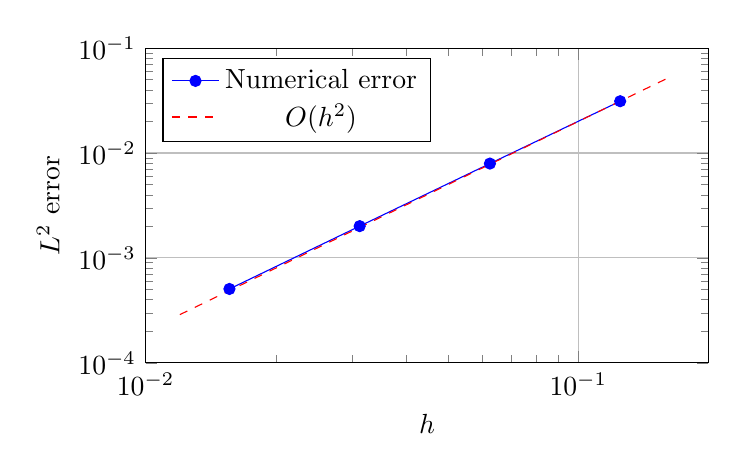
\begin{tikzpicture}
\begin{loglogaxis}[
  width=0.72\textwidth, height=0.46\textwidth,
  xlabel={$h$}, ylabel={$L^2$ error},
  grid=major, legend pos=north west,
  xmin=0.01, xmax=0.2, ymin=1e-4, ymax=1e-1]
\addplot[mark=*,blue] coordinates {
  (0.125,0.0312) (0.0625,0.00794) (0.03125,0.00201) (0.015625,0.000506)};
\addplot[dashed,red,domain=0.012:0.16] {2*x^2};
\legend{Numerical error, $O(h^2)$}
\end{loglogaxis}
\end{tikzpicture}
\caption{$L^2$ 误差的收敛曲线（示例）}\label{fig:conv}
\end{figure}

\section{结果分析}

由表 \ref{tab:error} 可见，随着 $h$ 减半，$L^2$ 误差约降至原来的 $1/4$，
收敛阶稳定在 $2$ 附近，与命题 \ref{prop:cea} 结合插值估计得到的结论相符。
误差主要来源于空间离散；若改用更高次单元或自适应网格，可进一步提高计算效率。
